\subsection{Evolutionary and Population-Based Hybrids}

\paragraph{EvE (Evolutionary Explorer).}
\begin{figure}[H]
\centering
\fitfigure{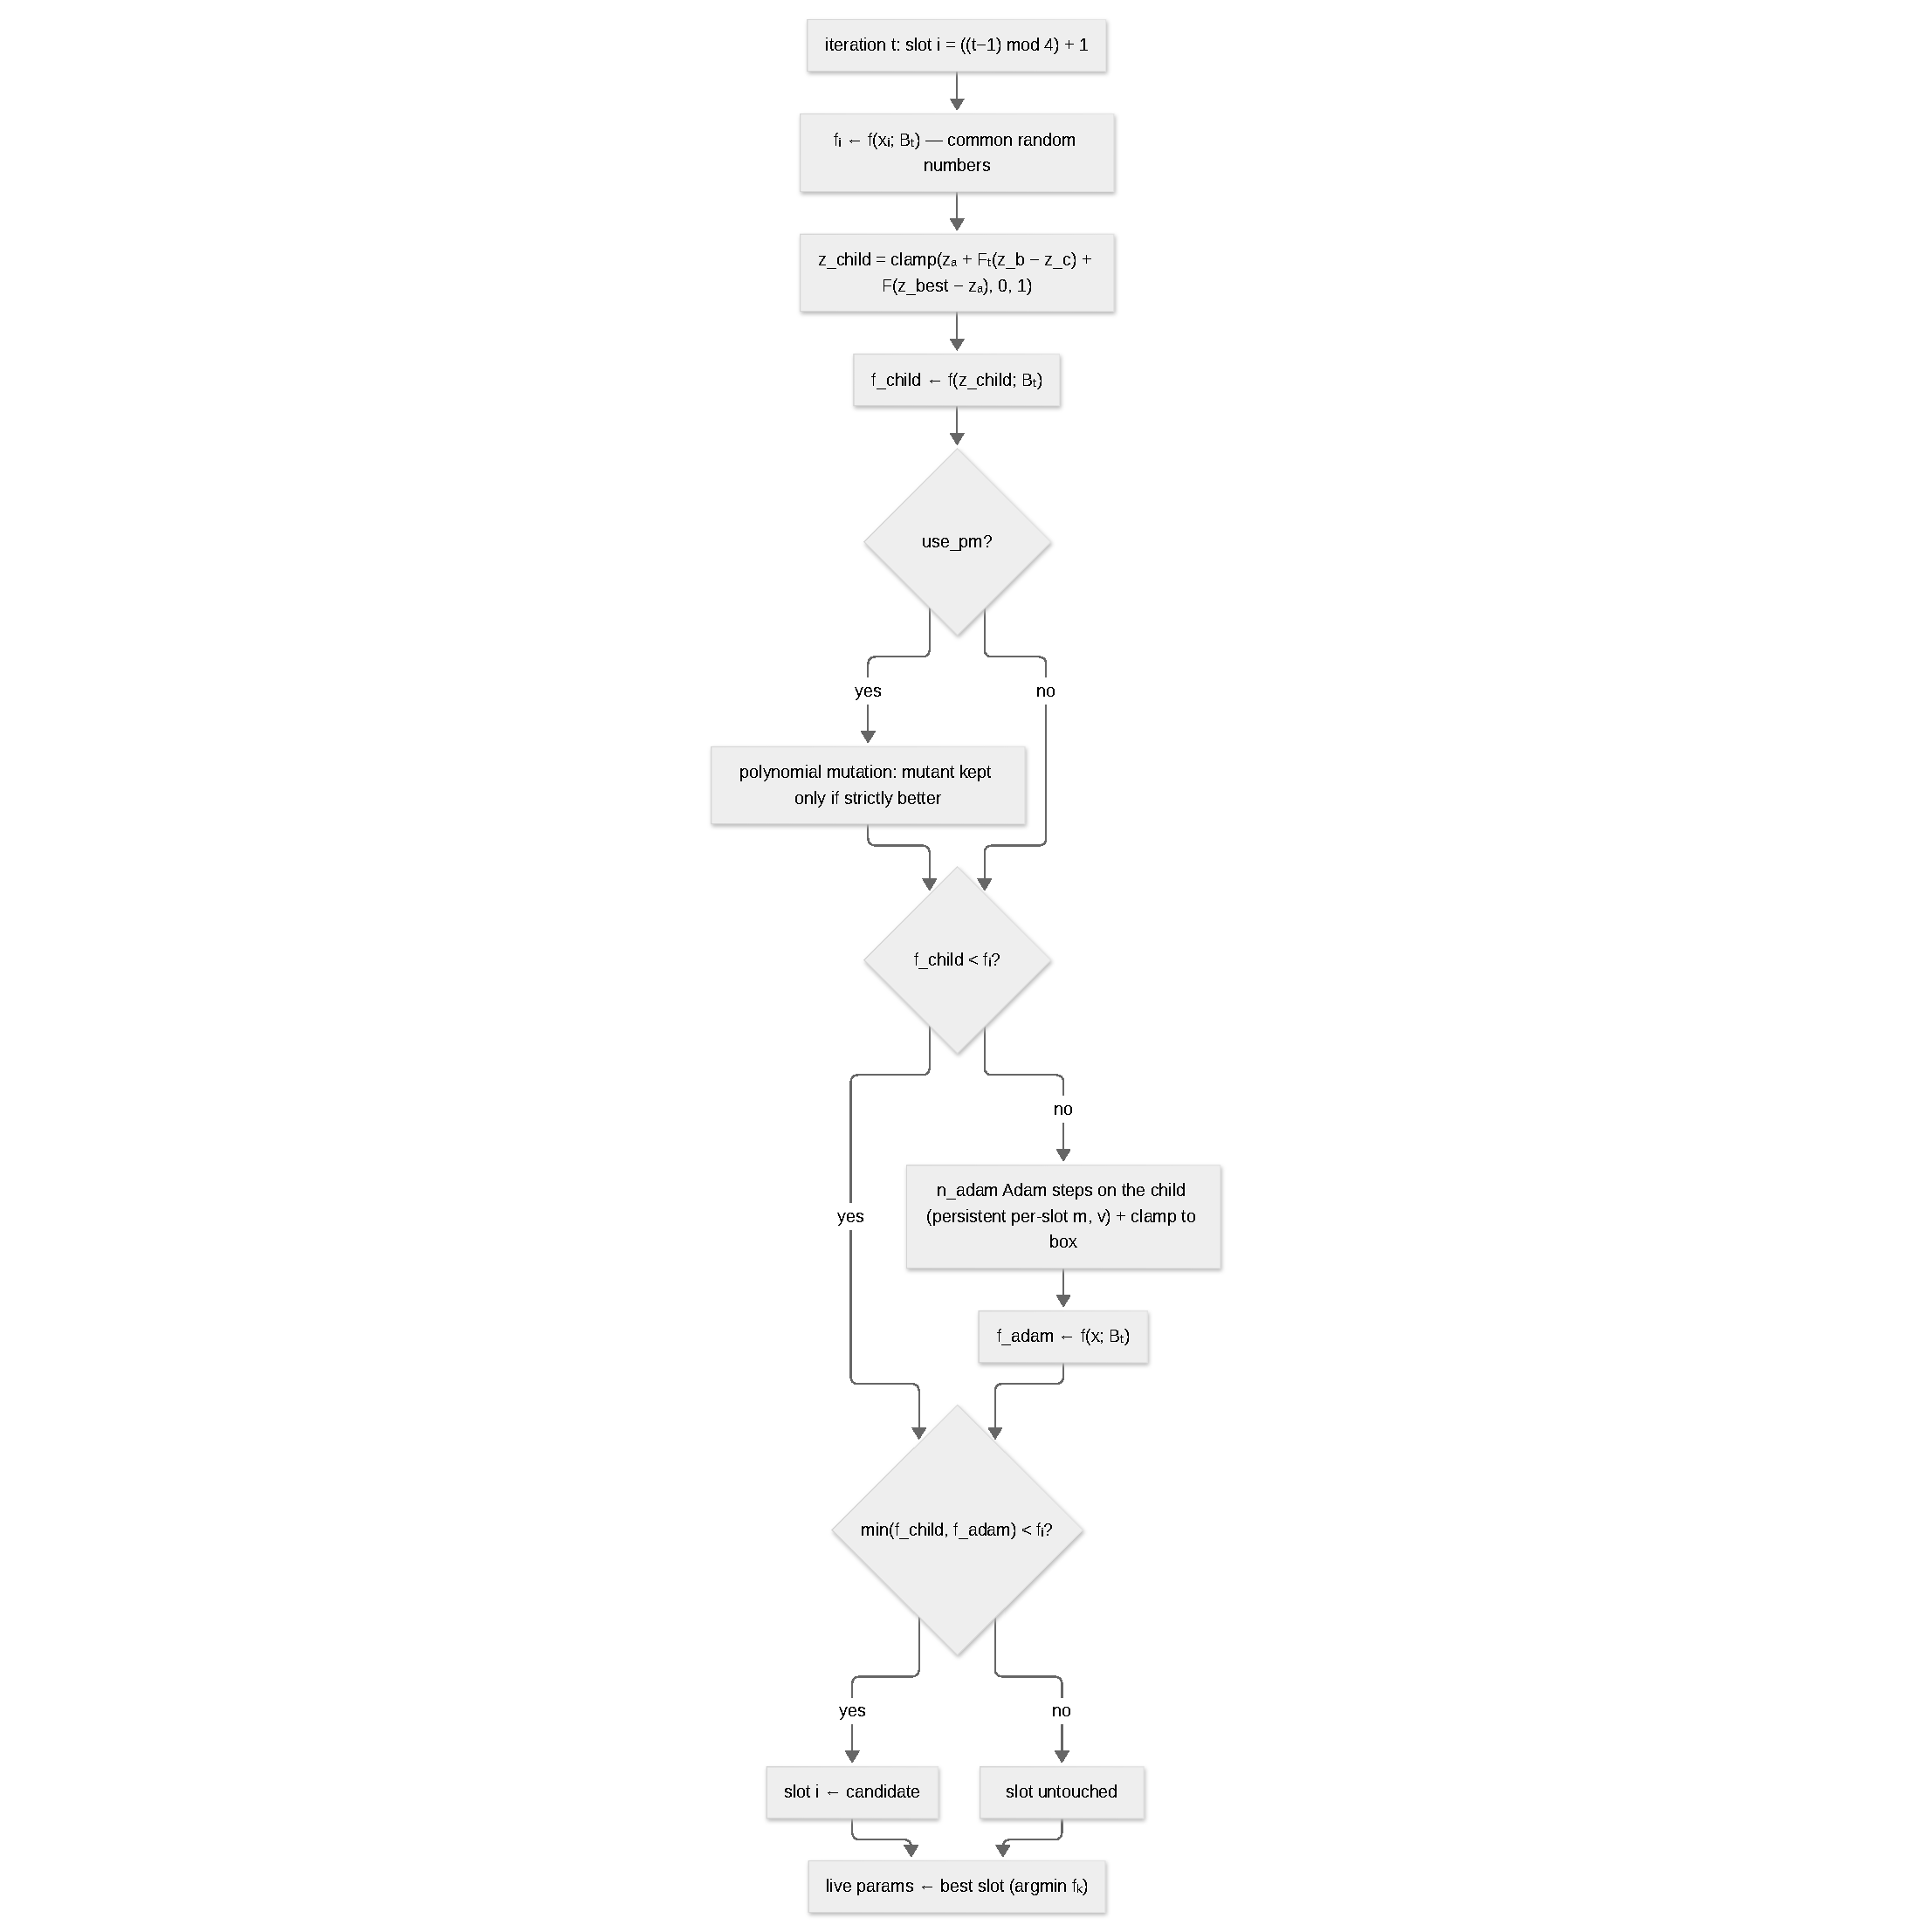
\includegraphics{figures/optimizers/eve.pdf}}
\caption{Step flow of EvE: a steady-state population of four challenges one round-robin slot per iteration with a DE child; a persistent-state Adam burst rescues the child only when it fails to improve, and greedy common-random-number selection keeps the best-so-far monotone.}
\label{fig:opt-eve}
\end{figure}
EvE~\citep{raj_eve_2026} is a \textbf{population-based alternate to Adam} targeted at the search-heavy, budget-constrained regime one level above final-stage training: ranking or pruning candidate configurations inside hyperparameter and architecture search. Instead of refining a single point, EvE keeps a steady-state population of four candidates and challenges one round-robin slot per iteration with a \emph{rand-to-pbest/1} differential-evolution child; only when the child fails to improve the slot's incumbent does EvE run a short burst of stock Adam on the same minibatch, keeping the refined point only if it beats the child. Selection is greedy, so the best-so-far value is monotone non-increasing on deterministic objectives, and because gradients are used only as a targeted rescue, per-iteration cost stays within a constant factor of a single Adam step regardless of dimension.

All internal search happens on the unit cube $z \in [0,1]^n$ via the affine map $\mathbf{x} = \mathbf{x}_l + \mathbf{z} \odot (\mathbf{x}_u - \mathbf{x}_l)$, so a fixed-size step never overshoots narrow-range coordinates or under-moves wide ones. The population is initialized by proximity — one anchor with three Gaussian jitters, $\sigma = 0.1$ — anchored at the model's own initial weights (the paper's LoRA precedent), with the per-tensor search box centered on the anchor at the Kaiming half-width $\sqrt{6/\mathrm{fan\_in}}$. Each iteration draws three distinct donors $a, b, c \ne i$ and builds the child with a jittered difference weight (the jitter applies only to the difference term; the pbest pull uses the unjittered $F$):
\begin{align}
z_{\text{child}} &= \operatorname{clamp}\big(z_a + F_t (z_b - z_c) + F (z_{\text{pbest}} - z_a),\ 0,\ 1\big), &
F_t &= F\big(1 + \gamma (u - \tfrac{1}{2})\big), \quad u \sim U(0,1),
\end{align}
with $F = 0.5$ and $\gamma = 10^{-4}$. An optional polynomial mutation (PM; off by default for neural-network training, since a single-coordinate nudge essentially never wins its accept/reject gate at network scale) perturbs exactly one gene at rate $p = 1/n$ with distribution index $\eta = 20$, the perturbation bounded and self-scaling to the distance to each boundary:
\begin{align}
z_d &\leftarrow z_d + \delta_q (z_u - z_l)_d, &
\delta_q &=
\begin{cases}
\bigl[2r + (1 - 2r)(1 - \delta_1)^{\frac{1}{\eta+1}}\bigr]^{\frac{1}{\eta+1}} - 1, & r \le 0.5,\\[2pt]
1 - \bigl[2(1 - r) + 2(r - 0.5)(1 - \delta_2)^{\frac{1}{\eta+1}}\bigr]^{\frac{1}{\eta+1}}, & r > 0.5,
\end{cases}
\end{align}
with $\delta_1 = (z_d - z_l)/(z_u - z_l)$, $\delta_2 = (z_u - z_d)/(z_u - z_l)$ and $r \sim U(0,1)$. When the (possibly mutated) child fails to beat the slot's value, EvE runs $n_{\text{adam}}$ stock-Adam steps on it \emph{in real coordinates}, with classic L2 weight decay folded into the gradient before the moment update (PyTorch's stock Adam, not AdamW's decoupled rule) and every iterate clamped back into the box:
\begin{align}
g_t &= \nabla_{\mathbf{x}} f(\mathbf{x}_{t-1}; B_t) + \lambda \mathbf{x}_{t-1}, &
m_t &= \beta_1 m_{t-1} + (1 - \beta_1) g_t, &
v_t &= \beta_2 v_{t-1} + (1 - \beta_2) g_t^2, \\
\widehat{m}_t &= \frac{m_t}{1 - \beta_1^t}, &
\widehat{v}_t &= \frac{v_t}{1 - \beta_2^t}, &
\mathbf{x}_t &= \operatorname{clamp}\Big(\mathbf{x}_{t-1} - \eta_{lr} \frac{\widehat{m}_t}{\sqrt{\widehat{v}_t} + \epsilon},\ \mathbf{x}_l,\ \mathbf{x}_u\Big),
\end{align}
with $\beta_1 = 0.9$, $\beta_2 = 0.999$, $\epsilon = 10^{-8}$. Each population slot keeps its own persistent $(m, v, t)$ state across the whole run, so fallback bursts form one continuous Adam trajectory rather than repeated cold starts. Every evaluation of an iteration — the slot refresh, the child and the whole fallback burst — is scored on one freshly drawn minibatch $B_t$ (common random numbers), and a candidate replaces the incumbent only if it is strictly better on that same batch. In this implementation the shared per-group \texttt{lr\_*}, \texttt{wd\_*}, \texttt{betas\_*} and \texttt{eps\_*} configure the Adam fallback per parameter group (\texttt{wd\_*} is the L2 term $\lambda$ inside $g_t$), the live model parameters always hold the best-so-far slot between steps, and the step is closure-based — the trainer re-evaluates the current batch on each candidate point inside \texttt{optimizer.step()}, which is why EvE requires \texttt{gradient\_accumulation\_steps: 1} and is not available for SBERT.

\begin{algorithm}[H]
\caption{EvE (Evolutionary Explorer)}
\label{alg:eve}
\begin{algorithmic}[1]
\Require Objective $f$ with bounds $\mathbf{x}_l, \mathbf{x}_u$, iterations $T$, DE weight $F$, jitter $\gamma$, init jitter $\sigma$, PM index $\eta$, fallback steps $n_{\text{adam}}$, fallback LR $\eta_{lr}$, L2 decay $\lambda$, seed $s$, USE\_PM
\Ensure Best point $\arg\min_k z_k$ and value $\min_k f_k$
\State $z_1 \sim U(0,1)^n$ (anchor: the initial weights); $z_k \gets \operatorname{clamp}(z_1 + \sigma\epsilon_k, 0, 1)$, $\epsilon_k \sim \mathcal{N}(0, I_n)$, $k = 2,3,4$ \Comment{Proximity init}
\State $f_k \gets f(\mathbf{x}_l + z_k \odot (\mathbf{x}_u - \mathbf{x}_l))$ for $k = 1,\dots,4$; $\text{state}_k \gets (\mathbf{0}, \mathbf{0}, 0)$ \Comment{Persistent Adam moments}
\For{$t = 1, \ldots, T$}
    \State $i \gets ((t - 1) \bmod 4) + 1$ \Comment{Round-robin target slot}
    \State draw minibatch $B_t$; $f_i \gets f(\mathbf{x}_i; B_t)$ \Comment{Common random numbers}
    \State draw distinct $a, b, c \in \{1,\dots,4\} \setminus \{i\}$; $F_t \gets F(1 + \gamma(u - 0.5))$, $u \sim U(0,1)$
    \State $z_{\text{child}} \gets \operatorname{clamp}(z_a + F_t(z_b - z_c) + F(z_{\text{pbest}} - z_a), 0, 1)$
    \State $f_{\text{child}} \gets f(z_{\text{child}}; B_t)$
    \If{USE\_PM} \Comment{PM's own accept/reject gate}
        \State $z_{\text{mut}} \gets \operatorname{PM}(z_{\text{child}}, \eta)$; $f_{\text{mut}} \gets f(z_{\text{mut}}; B_t)$
        \If{$f_{\text{mut}} < f_{\text{child}}$} $z_{\text{child}}, f_{\text{child}} \gets z_{\text{mut}}, f_{\text{mut}}$ \EndIf
    \EndIf
    \If{$f_{\text{child}} < f_i$}
        \State $z_{\text{cand}}, f_{\text{cand}} \gets z_{\text{child}}, f_{\text{child}}$
    \Else
        \State $\mathbf{x} \gets \mathbf{x}_l + z_{\text{child}} \odot (\mathbf{x}_u - \mathbf{x}_l)$
        \For{$n = 1, \ldots, n_{\text{adam}}$} \Comment{Targeted Adam fallback}
            \State $\mathbf{x} \gets \operatorname{AdamStep}(\mathbf{x}, \nabla_{\mathbf{x}} f(\mathbf{x}; B_t), \eta_{lr}, \lambda, \text{state}_i)$; \quad $\mathbf{x} \gets \operatorname{clamp}(\mathbf{x}, \mathbf{x}_l, \mathbf{x}_u)$
        \EndFor
        \State $z_{\text{adam}} \gets (\mathbf{x} - \mathbf{x}_l)/(\mathbf{x}_u - \mathbf{x}_l)$; \quad $f_{\text{adam}} \gets f(z_{\text{adam}}; B_t)$
        \State $(z_{\text{cand}}, f_{\text{cand}}) \gets \arg\min_{(z, f) \in \{(z_{\text{child}}, f_{\text{child}}),\, (z_{\text{adam}}, f_{\text{adam}})\}} f$
    \EndIf
    \If{$f_{\text{cand}} < f_i$} $z_i \gets z_{\text{cand}}$; \quad $f_i \gets f_{\text{cand}}$ \Comment{Greedy selection} \EndIf
\EndFor
\State \Return $\arg\min_k z_k$, $\min_k f_k$
\end{algorithmic}
\end{algorithm}

\paragraph{Cons.}
\begin{itemize}[leftmargin=*]
\item A step behind Adam at matched evaluation budgets: roughly one accuracy point on MNIST and 9--11\% higher relative test loss on the LoRA fine-tuning tasks; the paper does not claim final-stage superiority.
\item 13$\times$ the live parameter count in total storage (four population copies plus eight persistent moment copies) against Adam's 4$\times$; the measured peak GPU multiplier is lower (2.95$\times$) but fixed and dimension-independent.
\item The learning rate does not transfer from Adam's and needs its own search (3--100$\times$ higher depending on the task); the four-member population shows the widest seed-to-seed variance of the nine methods compared.
\item Closure-based step: the trainer re-evaluates the batch inside \texttt{optimizer.step()}, so gradient accumulation is unsupported and the SBERT loop (sentence-transformers \texttt{fit}) cannot host it; polynomial mutation is pure cost at network scale and is off by default.
\end{itemize}

\paragraph{Pros.}
\begin{itemize}[leftmargin=*]
\item Monotone best-so-far by construction on deterministic objectives (greedy accept-only-if-better selection), with per-iteration cost within a constant factor of a single Adam step regardless of dimension.
\item Wins or ties Adam on 76\% of 70 (problem, dimension) benchmark cells across seven classical scalable problems up to $10^6$ variables, most decisively on the multimodal ones.
\item Finishes matched evaluation budgets 1.7--3.9$\times$ faster in wall-clock on real training (an MLP on MNIST and LoRA fine-tuning of a 1.5B-parameter model), trading a modest amount of final quality for speed.
\item Inside successive halving, completes hyperparameter and architecture searches 3.1--3.5$\times$ faster while ranking candidate configurations about as consistently with Adam as Adam does with itself across seeds (Kendall's $\tau$ of 0.66--0.69).
\end{itemize}

\paragraph{EA4LLM (Evolution Strategies for Large Language Models).}
\begin{figure}[H]
\centering
\fitfigure{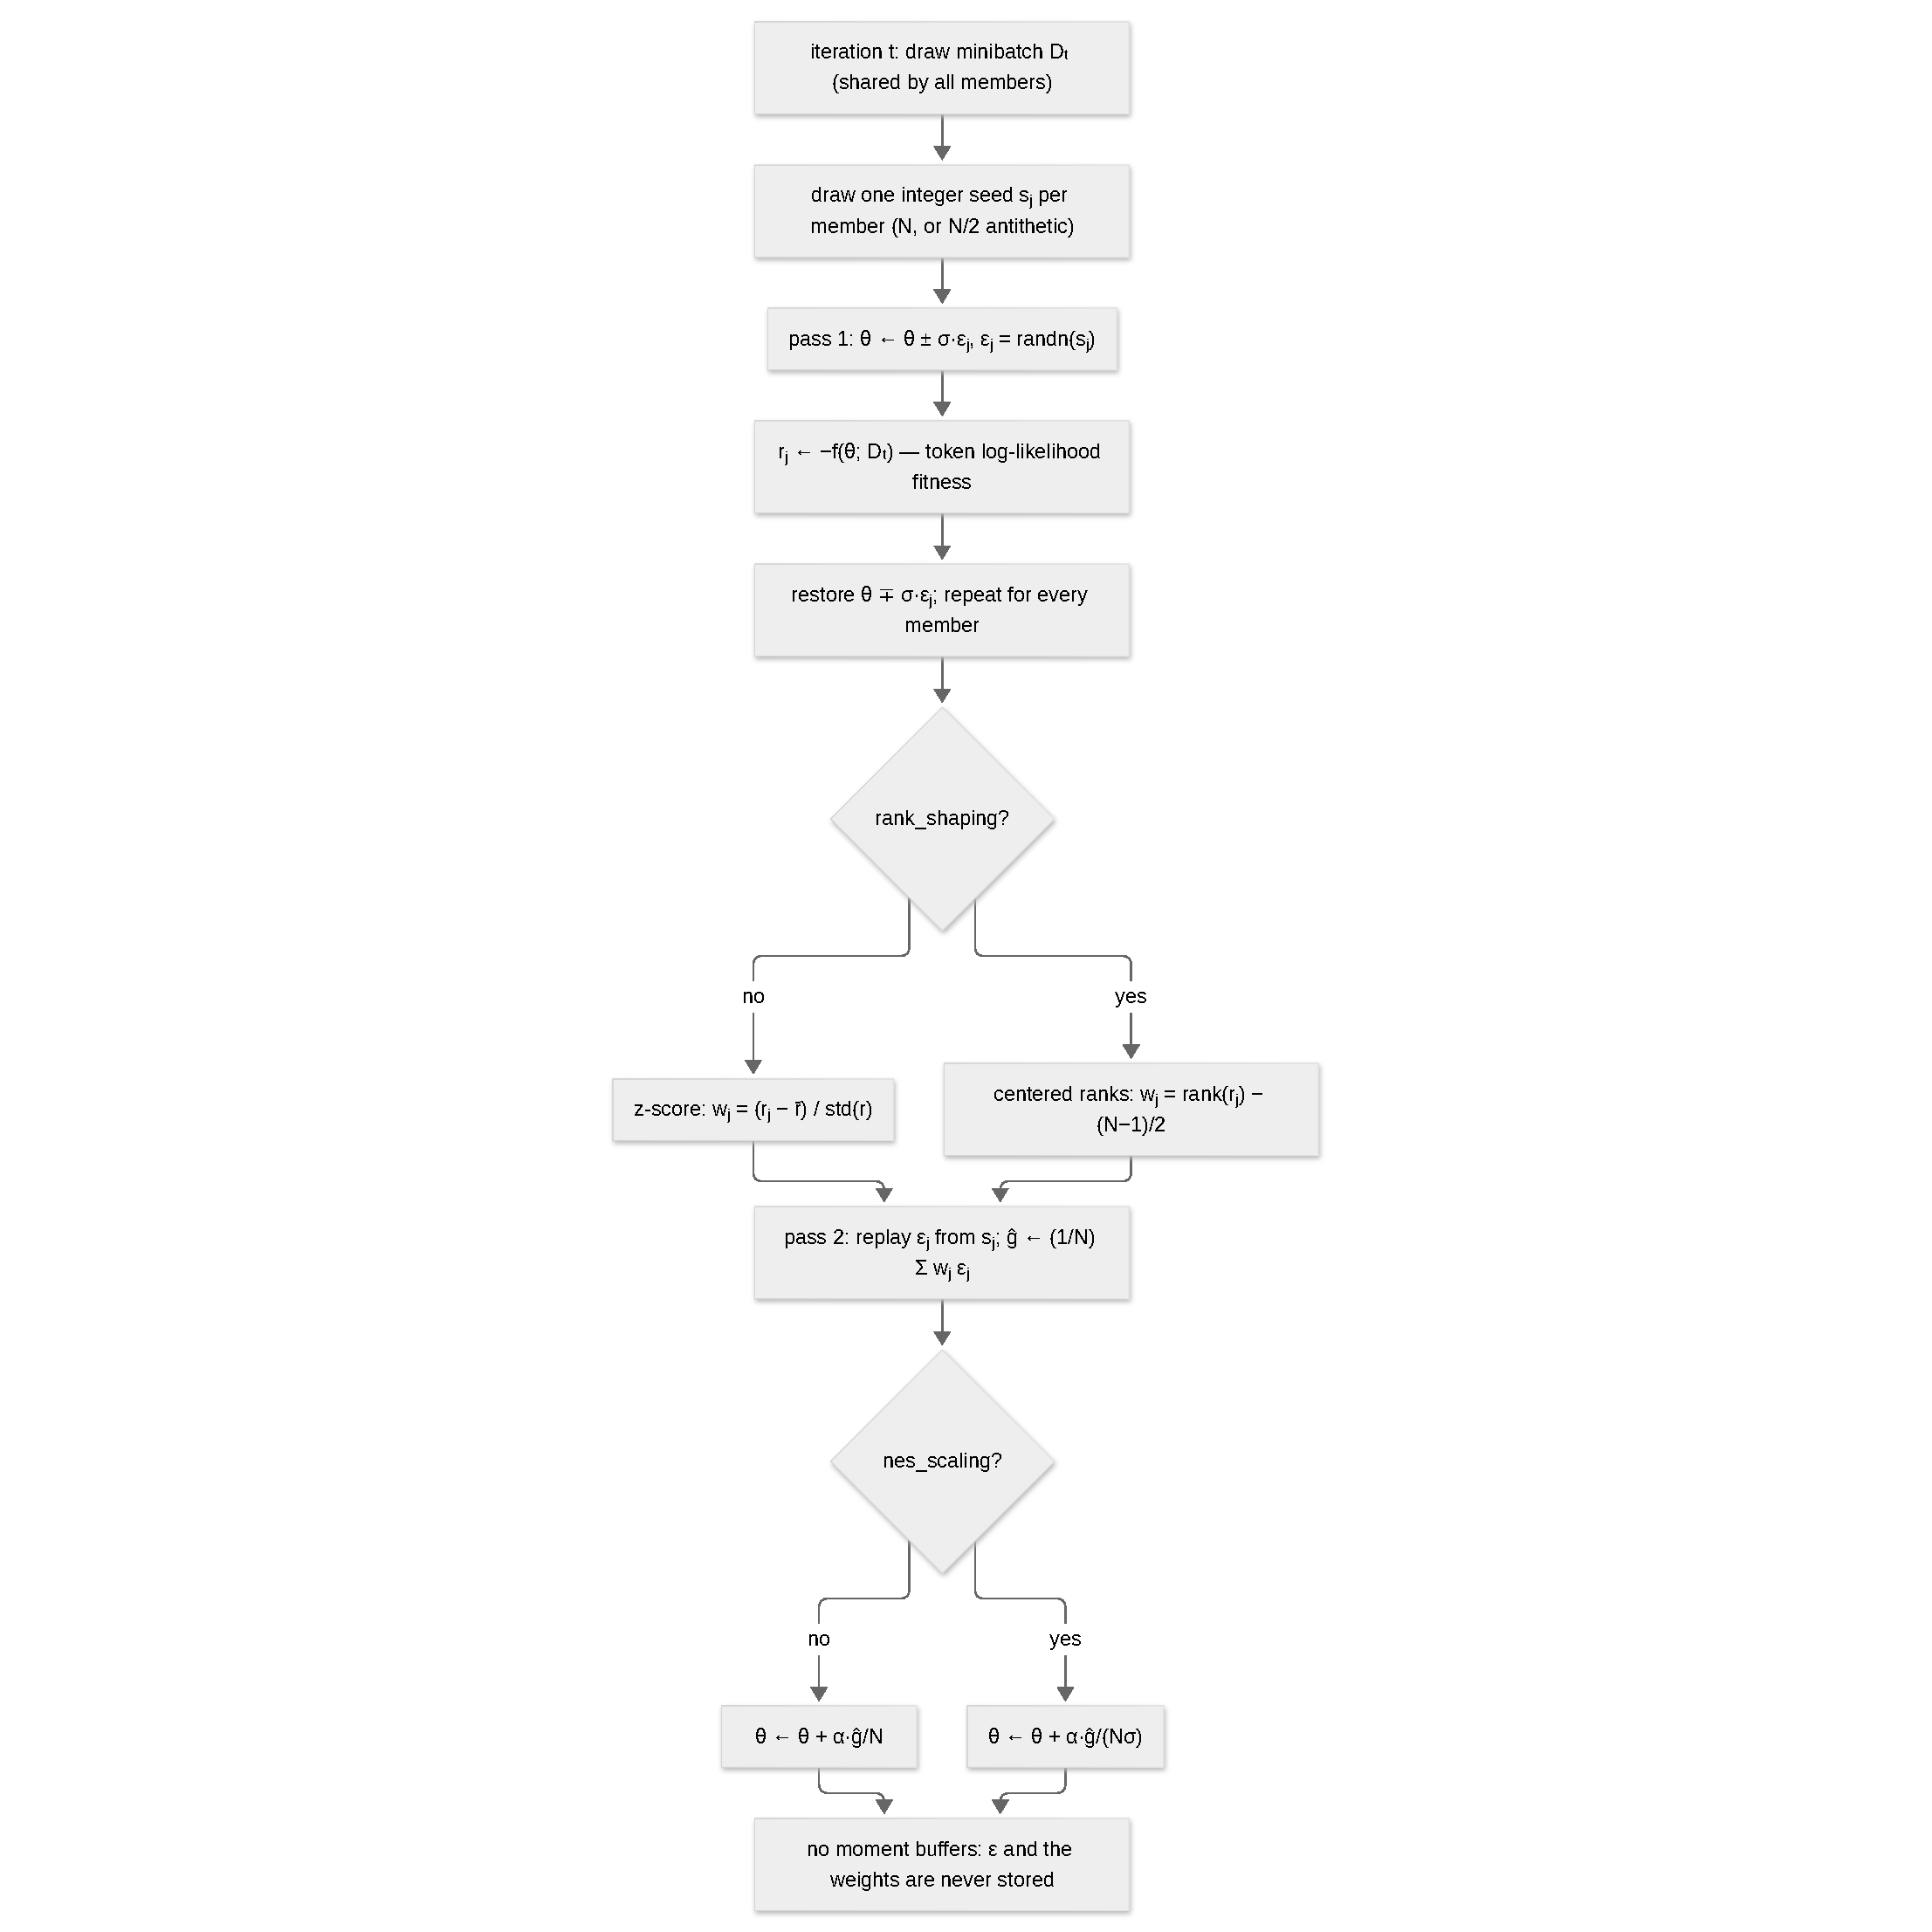
\includegraphics{figures/optimizers/ea4llm.pdf}}
\caption{Step flow of EA4LLM: each iteration evaluates $N$ Gaussian perturbations of the parameters on one minibatch shared by every member, scores them by the negated token-level log-likelihood, shapes the rewards into z-score or centered-rank weights, and replays the same seeded noise to accumulate the ES direction --- no gradients and no per-parameter optimizer state.}
\label{fig:opt-ea4llm}
\end{figure}
EA4LLM~\citep{liu_ea4llm_2025} is a \textbf{gradient-free alternative to Adam} that removes backpropagation and optimizer state entirely, and it is the first method the authors validate for full-parameter pretraining of LLMs from scratch, across Qwen3-style models from 0.5B to 32B parameters. Instead of differentiating a loss, EA4LLM treats the next-token likelihood as a black-box fitness and estimates a descent direction from a population of Gaussian perturbations. The fitness is the mean token-level log-probability of the true next token, masked for padding, which is exactly the standard causal-LM objective up to sign:
\begin{align}
p_t &= \operatorname{softmax}(z_t), &
R(x;\theta) &= \frac{1}{\sum_t m_t}\sum_{t=1}^{T} m_t \log p_\theta\!\left(x_{t+1}\mid x_{\le t}\right), &
F(\theta) &= \frac{1}{|D|}\sum_{x\in D} R(x;\theta),
\end{align}
with logits $z_t$, padding mask $m_t \in \{0,1\}$ and corpus $D$. Each iteration samples $N$ independent noises $\epsilon_j \sim \mathcal{N}(0, I)$, evaluates the perturbed fitness $r_j = F(\theta + \sigma\epsilon_j)$ on one uniformly drawn subset $D_t \subset D$ of size $M$ (the subset is shared by every member of the iteration, so the stochastic estimator stays unbiased, $\mathbb{E}[F_M(\theta)] = F(\theta)$), and shapes the rewards into weights by z-score normalization or centered ranks:
\begin{align}
w_j &= \frac{r_j - \bar r}{\operatorname{std}(r)}
&&\text{or}&
w_j &= \operatorname{rank}(r_j) - \frac{N-1}{2},
\end{align}
where $\operatorname{rank}(\cdot)$ assigns $0,\dots,N-1$ after sorting. The direction is the noise-weighted mean, optionally scaled NES-style by $1/\sigma$, and the update ascends the fitness:
\begin{align}
\hat g &= \frac{1}{N}\sum_{j=1}^{N} w_j \epsilon_j
&&\text{or}&
\hat g &= \frac{1}{N\sigma}\sum_{j=1}^{N} w_j \epsilon_j,
&&&
\theta \leftarrow \theta + \alpha \hat g .
\end{align}
Antithetic sampling evaluates the $\pm\sigma\epsilon$ pair of $N/2$ seeds instead of one sign per seed. The paper's runner uses $N = 30$, $\sigma = 10^{-3}$, $\alpha = 5\times 10^{-4}$ and $M = 5000$ evaluation samples per iteration ($T = 1000$ iterations, micro-batch 16, maximum sequence length 256); antithetic sampling, rank shaping, the NES $1/\sigma$ scaling, grouped/layered multipliers and step-size schedules are all \emph{off} in those runs, and Appendix~A.1 states that the deployed algorithm removes the grouped operators and multipliers outright. In this implementation the step is closure-based: the trainer's current minibatch supplies $D_t$ and the loss is negated to form the fitness, the shared per-group \texttt{lr\_*} is the step size $\alpha$, and \texttt{wd\_*} applies a decoupled multiplicative decay before the ES move (a repo-consistency extension --- the paper defines no weight decay). Noise is regenerated from one integer seed per member in a second pass, so the full noise set is never stored: optimizer state is O(1) and no moment buffers exist. Like EvE, EA4LLM requires \texttt{gradient\_accumulation\_steps: 1} and is not available for SBERT (the closure cannot coexist with the SBERT fit loop), and AMP is not supported on the closure path.

\begin{algorithm}[H]
\caption{EA4LLM (Zeroth-Order Evolution Strategies)}
\label{alg:ea4llm}
\begin{algorithmic}[1]
\Require Parameters $\theta$, fitness $F$ (negated loss), iterations $T$, population $N$, noise scale $\sigma$, step size $\alpha$, subset size $M$, normalization (z-score or rank), seed $s$, USE\_ANTITHETIC, USE\_RANK, USE\_NES
\Ensure Optimized parameters $\theta_T$
\State seed the persistent generator with $s$
\For{$t = 1, \ldots, T$}
    \State draw minibatch $D_t \subset D$, $|D_t| = M$ \Comment{Shared by all members}
    \State draw seeds $\{s_j\}_{j=1}^{N/2}$ (antithetic) or $\{s_j\}_{j=1}^{N}$
    \State $\text{rewards} \gets [\,]$ \Comment{Pass 1: perturb, evaluate, restore}
    \For{each seed $s_j$ and sign $\pm$ (or a single sign)}
        \State $\epsilon \gets \operatorname{randn}(s_j)$; \quad $\theta \gets \theta \pm \sigma\epsilon$; \quad $r \gets -f(\theta; D_t)$; \quad $\theta \gets \theta \mp \sigma\epsilon$
        \State append $r$ to rewards
    \EndFor
    \State $w \gets$ z-score(rewards) or centered ranks(rewards)
    \State $g \gets 0$ \Comment{Pass 2: replay the same noise}
    \For{each seed $s_j$ and sign $\pm$ (or a single sign)}
        \State $\epsilon \gets \operatorname{randn}(s_j)$; \quad $g \gets g + w_j (\pm\epsilon)$
    \EndFor
    \State $\theta \gets \theta + \alpha g / (N\sigma)$ if USE\_NES, else $\theta \gets \theta + \alpha g / N$
\EndFor
\State \Return $\theta_T$
\end{algorithmic}
\end{algorithm}

\paragraph{Cons.}
\begin{itemize}[leftmargin=*]
\item Requires $N$ forward evaluations per step (30 in the paper), so sample efficiency trails first-order methods and the variance of the estimate is higher; the paper reports sensitivity to $N$, $\sigma$, $\alpha$ and the normalization choice.
\item No gradient is available, so the gradient-clipping and AMP paths do not apply: the trainer's closure harness rejects \texttt{use\_amp}, requires \texttt{gradient\_accumulation\_steps: 1}, and the SBERT loop cannot host it. Each evaluation also pays a backward pass through the shared closure even though ES discards it.
\item At matched evaluation budgets the paper does not claim superior final quality to Adam; its case is memory (>4$\times$ reduction at $\ge$4B parameters) and gradient-free feasibility, with antithetic sampling, rank shaping and NES scaling disabled in its own large-scale runs.
\item Because the z-score makes the update magnitude independent of $\sigma$ and of the gradient scale, $\alpha$ must be tuned per task rather than transferred from Adam.
\end{itemize}

\paragraph{Pros.}
\begin{itemize}[leftmargin=*]
\item Zero optimizer state: no moments and no population copies, so the paper measures 60.01 vs 137.61~GB at 8B and 137.61 vs 431.76~GB at 32B against Adam.
\item Provides the first stable full-parameter ES pretraining from scratch across 0.5B--32B, with steadily decreasing loss curves (Figure~1) and no gradient computation.
\item Architecture-agnostic: the fitness only needs a forward pass and a probability, so non-differentiable operators become trainable.
\item The subsampled fitness is an unbiased estimator of the full-corpus fitness, and the two-pass seeded replay makes the noise reproducible while keeping optimizer state at O(1).
\end{itemize}

